\begin{tcolorbox}[title={\large 背景}]
	\structure{グラフ}は広く用いられる重要なデータ構造
	\vspace{15pt}
	\begin{easylist}[itemize]
	@ 化学構造式
	\vspace{10pt}
	@ RNA二次構造
	\vspace{10pt}
	@ 構文木 \\
	\end{easylist}
	\vspace{20pt}

	\structure{グラフに対する教師付き学習}
	\vspace{15pt}
	\begin{easylist}[itemize]
	@ 様々な分野での応用
	\vspace{10pt}
	@@ 創薬
	\vspace{10pt}
	@@ 材料科学
	\end{easylist}
	\vspace{105pt}
	\begin{textblock*}{\textwidth}(450pt,-180pt)
		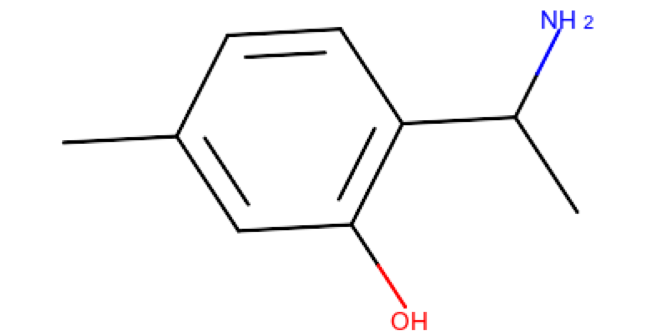
\includegraphics[width=330pt]{img/chemical.png}
	\end{textblock*}
	\begin{textblock*}{\textwidth}(800pt,-180pt)
		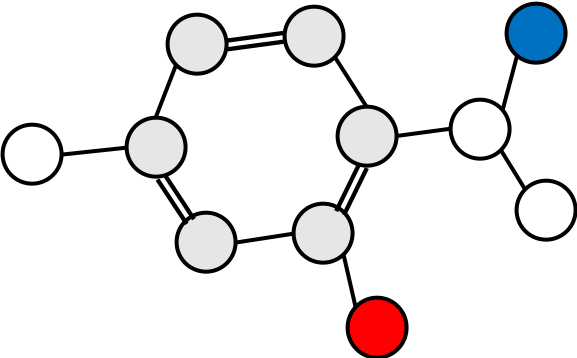
\includegraphics[width=260pt]{img/chemical_graph.png}
	\end{textblock*}
\end{tcolorbox}
